\newcommand{\text}[1]{\mbox{#1}}
\newcommand{\impl}{\Rightarrow}
\newcommand{\et}{\wedge}
\newcommand{\ou}{\vee}
\newcommand{\define}{\Leftrightarrow{def}}
\newcommand{\mssi}{\Leftrightarrow}

\newcommand{\llb}{\llbracket}
\newcommand{\ch}[1]{[#1]}
\newcommand{\mch}[1]{[#1[}
\newcommand{\allch}[1]{\llb #1] }
\newcommand{\allmch}[1]{\llb #1[}

\newcommand{\n}[1]{\ensuremath{\mathfrak{#1}}}
\newcommand{\nE}{\n{E}}
\renewcommand{\P}[1]{\ensuremath{\mathit{P}(\n{#1})}}
\newcommand{\D}[2]{\ensuremath{\mathit{D}(\n{#1},\n{#2})}}
\newcommand{\Pd}[1]{\ensuremath{\mathit{Pd}(\n{#1})}}
\newcommand{\Pdi}[1]{\ensuremath{\mathit{Pd}^{\infty}(\n{#1})}}
\newcommand{\Pda}[1]{\ensuremath{\mathit{Pd}^{+}(\n{#1})}}
\newcommand{\dpdc}[1]{\ensuremath{\mathit{DpdC}(\n{#1})}}
\newcommand{\codpdc}[1]{\ensuremath{\mathit{CoDpdC}(\n{#1})}}
\renewcommand{\succ}[1]{\ensuremath{\mathit{Succ}(\n{#1})}}
\newcommand{\succl}[1]{\ensuremath{\mathit{Succ_{L}}(\n{#1})}}

\newcommand{\ssi}{si et seulement si }

\chapter{Dépendances de contrôle}\label{sec-cdg}

\section{Introduction}

Intuitivement, un noeud \n{n} du PDG a une dépendance de contrôle sur un noeud
\n{c}
si le fait d'exécuter \n{n} dépend du résultat de l'exécution de \n{c}.
Typiquement, \n{c} est un noeud qui a plusieurs successeurs, comme un {\sc if} par
exemple,
et en fonction de la branche qui est choisie, \n{n} est exécuté ou non.

Nous allons voir qu'il existe de nombreuses façons de calculer ces
dépendances de contrôle, mais que nous avons du les adapter car
elle ne correspondent pas exactement à ce que l'on souhaitait faire.
Le principal problème est que
nous nous proposons d'analyser correctement
toute fonction, même en présence de sauts quelconques, voire de boucles
infinies; ce qui, comme nous allons le voir,
pose des problèmes particuliers au niveau des dépendances de contrôle.

\section{Etat de l'art}

Commençons tout d'abord par rappeler quelques définitions
et rapporter les résultats que l'on trouve dans la littérature.

\subsection{CFG}

Le \indexdef{graphe de flot de contrôle} est un graphe orienté qui définit l'ordre
d'exécution des instructions. Un noeud \n{a} est connecté à un noeud \n{b}
si l'instruction \n{b} peut suivre immédiatement
l'instruction \n{a} dans une trace l'exécution.
On dit que \n{b} est un \indexdef{successeur} de \n{a}.
On représente l'ensemble des successeurs d'un noeud \n{a} par $\succ{a}$.
On dit aussi que \n{a} est un \indexdef{prédécesseur} de \n{b}.\\

Un noeud est considéré comme une entrée dans le CFG s'il n'a pas de prédécesseur.
Il est généralement considéré qu'il y a un unique noeud d'entrée,
et que tous les noeuds du CFG sont atteignables depuis ce point d'entrée.
Cette hypothèse semble raisonnable car on s'intéresse au CFG d'une fonction
qui a bien un seul point d'entrée, et les instructions non atteignables depuis
le point d'entrée sont du
code mort que l'on peut donc ignorer dans les analyses.\\

Un noeud est considéré comme une sortie du CFG s'il n'a pas de successeur.
Son unicité et son accessibilité sont discutées plus loin.


\subsection{Postdominateurs}

La plupart des algorithmes de calcul des dépendances de contrôle
se basent
sur un CFG dans lequel sont ajoutés deux noeuds spéciaux {\sc start} et
{\sc stop} (on notera \nE{} ce dernier),
et sur la notion de  \indexdef{postdominateur} dont une définition est
la suivante~:

\begin{definition}{postdominateur}
  Une instruction \n{a} est {\bf postdominée} par une instruction \n{b}
  (\n{b} est un {\bf postdominateur} de \n{a})
  si tous les chemins qui vont de \n{a} au noeud \nE{} contiennent \n{b}.
\end{definition}

En d'autres termes, si on passe par l'instruction \n{a},
on passe forcement par tous ses postdominateurs avant de sortir.
Ou encore,
toutes les traces partant de \n{a} et allant à \nE{} passent par \n{b}.\\


Certains auteurs définissent également
le \indextxtdef{premier postdominateur}{postdominateur!premier}
(appelé aussi \indextxtdef{postdominateur immédiat}{postdominateur!immédiat})
de la façon suivante~:

\begin{definition}{premier postdominateur}
  \n{b} est le premier postdominateur de \n{a} \ssi~:
\begin{itemize}
  \item \n{b} postdomine \n{a},
  \item et \n{b} est postdominé par tous les autres postdominateurs de \n{a}.
\end{itemize}
\n{b} est donc unique.
\end{definition}

Cela permet de construire un arbre (appelé PDT pour {\it Post-Dominator Tree})
représentant cette relation dans lequel les noeuds sont les mêmes que
ceux du CFG et le père de chaque noeud est son premier postdominateur.\\

L'ensemble des postdominateurs d'un noeud \n{a} est donné par~:
$$
\Pd{a} = \{a\} \bigcup \bigcap_{s \in \succ{a}} \Pd{s}
$$
qui traduit le fait que \n{b} postdomine \n{a} \ssi $\n{b} = \n{a}$
ou \n{b} postdomine tous les successeurs de \n{a}.
La méthode de calcul consiste à initialiser tous les ensembles à $\top$,
et à itérer jusqu'à stabilisation.
La fonction étant décroissante, la convergence est assurée.\\


La notion classique de postdominateurs suppose que le CFG ait un point unique de
sortie \nE,
et que celui-ci soit atteignable depuis tous les autres points du graphe.
Si ce n'est pas le cas, à la fin de ce calcul,
pour les \n{a} n'ayant pas de chemin vers \nE, on a~: $\Pd{a} = \top$.\\


\subsection{Dépendances de contrôle}

Intuitivement, on dit qu'une instruction \n{a} a une \indextxtdef{dépendance de
contrôle}{dépendance!contrôle} sur une instruction \n{c}
si, en fonction du choix que l'on fait en \n{c}, on passe ou non en \n{a}.
Cela suppose donc qu'il y ait un choix à faire en \n{c},
c'est-à-dire que le noeud correspondant dans le CFG
ait plusieurs successeurs.\\

Les dépendances de contrôle sont définies par \cite{Ferrante87}
de la façon suivante~:

\begin{definition}{dépendances de contrôle selon \cite{Ferrante87}}
  Pour deux noeuds \n{a} et \n{b} du CFG, \n{b} dépend de \n{a} ssi~:
\begin{itemize}
  \item il existe un chemin P de \n{a} a \n{b}
    tel que tout noeud Z de P, différent de \n{a} et de \n{b}, est postdominé
    par \n{b},
  \item et \n{a} n'est pas postdominé par \n{b}.
\end{itemize}
\end{definition}

Ce qui signifie que~:
\begin{itemize}
  \item plusieurs chemins partent de \n{a},
  \item qu'il existe un chemin qui passe par \n{b},
  \item et qu'il existe aussi un chemin qui ne passe pas par \n{b}
    (sinon, \n{a} serait postdominé par \n{b}).
\end{itemize}

Ce qui conduit à une autre
définition, équivalente à la précédente~:

\begin{definition}{dépendance de contrôle}
  Une instruction \n{b} a une {\bf dépendance de contrôle} vis à vis de \n{a} si~:
\begin{itemize}
  \item \n{b} postdomine certains successeurs de \n{a},
  \item \n{b} ne postdomine pas tous les successeurs de \n{a}.
\end{itemize}
\end{definition}

Pour calculer le CDG, l'algorithme de référence est le suivant~:

\begin{algo}{calcul du CDG selon \cite{Ferrante87}}
\begin{itemize}
\item soit ACFG le CFG (+ START et {\sc stop}) dans lequel sont ajoutés~:
  \begin{itemize}
    \item un noeud ENTRY,
    \item une arrête (ENTRY,START),
    \item une arrête (ENTRY,
      {\sc stop}),
  \end{itemize}
\item soit S l'ensemble des arrêtes (\n{a},\n{b}) de ACFG
  telles que \n{b} ne postdomine pas \n{a}, \\
  (c'est-à-dire les arrêtes partant des noeuds \n{a} qui ont plusieurs successeurs)
\item soit \n{l} le plus petit ancêtre commun à \n{a} et \n{b} dans PDT\\
  (on peut montrer que soit \n{l}=\n{a}, soit \n{l} est le père de \n{a} dans PDT)
  \begin{itemize}
    \item si \n{l} est le père de \n{a} dans PDT, tous les noeuds du PDT sur le chemin
      entre \n{l} et \n{b} (\n{b} compris, mais pas \n{l}) dépendent de \n{a},
    \item si \n{l} = \n{a}, tous les noeuds du PDT sur le chemin
      entre \n{a} et \n{b} (\n{a} et \n{b} compris) dépendent de \n{a}.
  \end{itemize}
\end{itemize}
En fait, il est plus simple de dire que  tous les noeuds du PDT sur le chemin
entre \n{b} et le père de \n{a} (\n{b} compris, mais pas le père de \n{a}) dépendent de
\n{a}.
\end{algo}

La relation de dépendance étant transitive, on peut choisir de calculer
uniquement les dépendances directes ou d'inclure les dépendances indirectes.

\begin{exemple}
\begin{tabular}{m{8cm}m{4cm}}
  Dans le CFG ci-contre, \n{b} a bien une dépendance de contrôle sur \n{a}.
  On remarque que, par contre, Z1 ou Z2 ne dépendent pas directement de \n{a},
  car ils ne postdominent pas S2. En revanche, il y a néanmoins une dépendance
  indirecte, comme on pouvait s'y attendre, car Z dépend de \n{a}, et Z1 et Z2
  dépendent de Z.
&
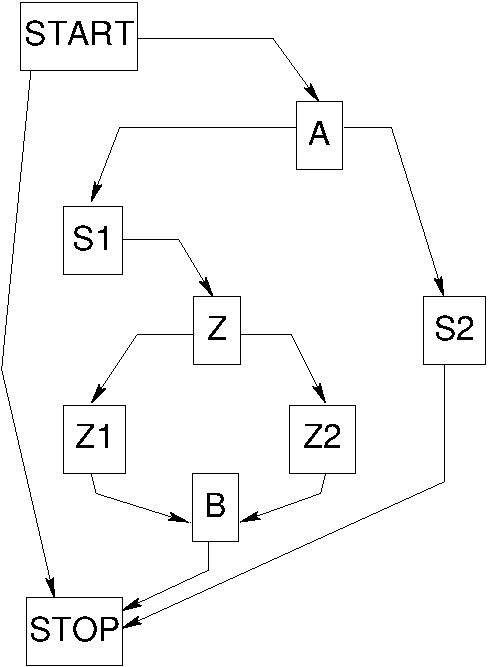
\includegraphics[width=4cm]{ctrl-dpds}
\end{tabular}
\end{exemple}

En fait, \n{a} dépend directement de c si
\n{a} est forcement atteint si on passe par l'un des successeurs de c,
mais il y a des chemins qui partent de c et qui ne passe pas pas \n{a}.

\subsection{Cas particuliers}

Ce qui a été présenté ci-dessus s'applique bien à des programmes bien
structurés, mais nécessite des adaptations si on s'intéresse~:

\begin{itemize}
  \item aux instructions qui modifie le flot de contrôle telles que les sauts,
  \item aux CFG qui contiennent des noeuds pour lesquels il n'y a pas de chemin
    vers le noeud de sortie.
\end{itemize}

Nous allons étudier plus précisément ces deux points ci-dessous.

\section{Nos définitions}

\subsection{Chemins}

Dans ce qui suit, on utilise beaucoup la notion de \indexdef{chemin}~:
un chemin est une liste de noeuds du CFG telle que si deux noeuds \n{a} et \n{b}
se suivent dans la liste, \n{b} est un successeur de \n{a}.
Nous appelons \indexdef{trace} un chemin qui se termine par un noeud
n'ayant pas de successeur, ou un chemin qui est infini.

On définit quelques notations pour désigner les chemins~:
\begin{itemize}
  \item $\ch{a, b}$  un chemin allant de \n{a} à \n{b}
  \item $\mch{a, b}$ une trace partant de \n{a} et passant par \n{b}
  \item $\mch{a, -}$ une trace partant de \n{a},
  \item $\ch{a, b, c}$ un chemin allant de \n{a} à \n{c} en passant par \n{b},
  \item $\ch{a;s, b}$
    un chemin allant de \n{a} à \n{b} en passant par $\n{s} \in \succ{a}$,
  \item $\mch{a, \neg b}$
    une trace partant de \n{a} et ne passant pas par \n{b},
\end{itemize}
et des ensembles de chemins :
\begin{itemize}
  \item $\allmch{a, -}$ toutes les traces partant de \n{a},
  \item $\allmch{a, b}$ toutes les traces partant de \n{a} et passant
    par \n{b},
  \item ...
\end{itemize}

On dit qu'un noeud appartient à un chemin, et on écrit - un peu abusivement -
$\n{x} \in \ch{a, b}$ si \n{x} apparaît au moins une fois
dans la liste qui décrit le chemin.

\subsection{Postdominateurs}

Avec les notations ci-dessus,
on peut définir \Pd{a} l'ensemble des postdominateurs de \n{a},
de la façon suivante~:
$$
  \n{b} \in \Pd{a} \define \forall t \in \allch{a, \nE}, \n{b} \in t
$$

On remarque que si on applique la définition ci-dessus à un CFG
qui contient des noeuds tels qu'il n'y a pas de chemin vers la sortie,
on a ~:
$$
\forall \n{a}, \allch{a, \nE} = \emptyset \impl \forall \n{b}, \n{b} \in \Pd{a}
$$
c'est-à-dire que l'on considère que de tels noeuds sont postdominés par tous les
autres, ce qui n'est pas très intéressant en terme de trace d'exécution~!\\

Dans ce qui suit, on note \P{a} l'ensemble des noeuds qui sont forcement
atteints quand on passe par \n{a},
et nous laisserons volontairement cette notion
un peu floue pour l'instant. Sa définition sera précisée en \S\ref{sec-pda}.

\subsection{Dépendances de contrôle} \label{sec-dpdc-if}

On définit \D{c}{s} comme
l'ensemble des noeuds qui sont forcement atteints si on passe par
\n{s}, mais pas forcement si on passe par \n{c}.
Plus formellement~:
$$
\D{c}{s} = \P{s} - \P{c}
$$
Par exemple, dans une séquence simple, si \n{c} représente un
\verbtt{if} et \n{s} la première instruction de l'une des branche, \D{c}{s}
donne les instructions de cette branche qui dépendent de la condition.\\

On définit alors $\dpdc{a}$,
l'ensemble des dépendances de contrôle de \n{a}, par~:
$$
\n{c} \in \dpdc{a} \define \n{a} \in \bigcup_{ \n{s} \in \succ{c}} \D{c}{s}
$$
Il est sans doute plus naturel de définir \codpdc{c},
l'ensemble des co-dépendances de contrôle de \n{c},
comme l'ensemble des noeuds ayant une dépendance de contrôle sur \n{c},
c'est-à-dire~:
$$
  \n{a} \in \codpdc{c} \define \n{c} \in \dpdc{a}
$$
On a alors~:
$$
\codpdc{c} = \bigcup_{ \n{s} \in \succ{c}}  \D{c}{s}
$$


On remarque que cette définition ne suppose pas que \n{c} ait plusieurs
successeurs, mais si \n{c} n'a qu'un successeur \n{s}~:
$$
\succ{c} = \{ \n{s} \} \impl
\codpdc{c} = \{\n{x} | (\exists t \in \allmch{c, -}, \n{x} \notin t)
\et (\forall t \in \allmch{s, -}, \n{x} \in t) \}
$$
or, comme \n{c} n'a qu'un successeur~:
$$
\forall t \in \allmch{c, -}, t = \mch{c; s, -}
$$
donc~:
$$
\forall t_s \in \allmch{s, -}, \n{x} \in t_s
\impl \forall t_c \in \allmch{c, -}, \n{x} \in t_c
$$
$$
\forall t_s \in \allmch{s, -}, \n{x} \in t_s
\impl \nexists t_c \in \allmch{c, -}, \n{x} \notin t_c
$$
et donc, finalement~:
$$
\succ{c} = \{ \n{s} \} \impl \codpdc{c} = \{\}
$$
Donc, un noeud n'ayant qu'un seul successeur ne peut pas être une dépendance de
contrôle. {\bf Attention}~: ceci n'est pas vrai pour les saut inconditionnels,
car ceux-ci donne lieu à un traitement spécial décrit en \S\ref{sec-goto}.


\section{Les sauts inconditionnels}\label{sec-goto}

\subsection{Présentation du problème}

Comme on l'a vu,
la définitions précédente des dépendances de contrôle conduit à
ne construire des dépendances que sur les noeuds ayant plusieurs successeurs,
c'est-à-dire ceux qui présente une forme de choix dans le CFG.
Or certaines instructions n'ayant qu'un successeur
peuvent aussi, par leur présence, modifier le flot de contrôle.
En C, c'est le cas par exemple des \verbtt{goto} explicites,
mais aussi des  \verbtt{break}, \verbtt{continue} ou \verbtt{return}.
Dans CIL, c'est aussi le cas des boucles puisqu'elles sont toutes transformées
en \verbtt{while(1)}.

Lorsque l'on souhaite utiliser le CDG pour calculer une réduction,
on aimerait
qu'il contienne également les liens nécessaires sur ces instructions
afin de déterminer si elles peuvent être supprimées,
ou si elles doivent être présentes dans le programme réduit.\\

L'exemple simple suivant, tiré de \cite{Choi94}, met en évidence ce problème~:

\begin{exemple}
\begin{tabular}{m{5cm}m{5cm}}
\begin{clisting}
1 : <entry>
2 : if (Q) goto 5;
3 : x = 4;
4 : goto 6;
5 : x = 5;
6 : y = x;
7 : <exit>
\end{clisting}
&
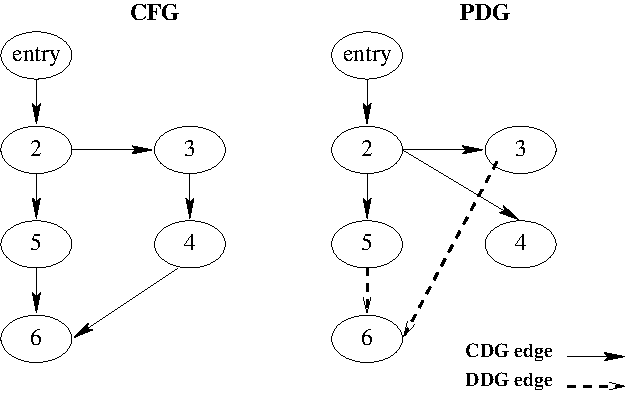
\includegraphics[width=5cm]{ex-goto}
\end{tabular}

\begin{tabular}{p{5cm} p{7cm}}
Réduction (fausse) \\
par rapport à <y,7>~:
\begin{clisting}
1 : <entry>
2 : if (Q) goto 5;
3 : x = 4;

5 : x = 5;
6 : y = x;
7 : <exit>
\end{clisting}
&
On voit que dans le graphe de dépendances (PDG), personne ne dépend de 4,
et la réduction de ce programme par rapport au noeud 6 donne le résultat
erroné ci-contre qui donne \verbtt{y=5} même lorsque $Q$ est faux.
\end{tabular}
\end{exemple}

\subsection{Etat de l'art}

La plupart des solutions proposées pour résoudre ce problème
utilisent la notion de \indexdef{successeur lexical} (sous différents noms).

\begin{definition}{successeur lexical immédiat  selon \cite{agrawal94slicing}}
A statement, S', is said to be {\bf the immediate lexical successor}
of a statement, S, in a program, if deleting S from the program
will cause the control to pass to S'
whenever it reaches the corresponding location in the new program.

If is a compound statement,
such as an If or a While statement, delleting means
delleting it allong with the statements that constitute its body.\\
\end{definition}

\cite{Choi94} présente une méthode qui ajoute un pseudo-lien dans le CFG
entre les \verbtt{goto} et leur successeur lexical immédiat,
et qui se sert de ce CFG modifié pour calculer les dépendances
de contrôle selon la méthode classique.
En fait, c'est un peu comme s'il remplaçait les \verb!goto L;!
par \verbtt{if (1) goto L;} pour mettre en évidence le chemin
qui apparaît dans le CFG si on supprime l'instruction.\\


\cite{agrawal94slicing} donne un algorithme qui permet de traiter
les \verbtt{goto} après un \slicing{} "normal".
Il s'agit, pour chaque \verbtt{goto} (G) non visible,
de déterminer si son premier postdominateur
présent dans la réduction est différent du premier successeur lexical.
Si c'est le cas, il faut rentre (G) visible ainsi que toutes ses dépendances.
Ceci donne les mêmes résultats que l'algorithme précédent,
mais il permet de ne modifier ni le CFG, ni le PDT.
Par contre, le calcul doit être fait pour chaque réduction.\\

\cite{harman98new} propose un algorithme qui donne des résultats
plus précis que les deux précédents dans certains cas.\\

Enfin, \cite{kumar02better} présente un algorithme qui prend
en compte le problème spécifique des \verbtt{switch} et donne
également de meilleurs résultats sur certains exemples.

\subsection{Discussion}\label{sec-dpdc-goto}

Dans un premier temps, l'algorithme de \cite{Choi94} semble simple à
implémenter, mais il nous oblige à calculer un nouveau CFG et le PDT
correspondant, ce que nous ne souhaitons pas faire car ces informations sont
utilisées par différents modules de l'outil.
Par ailleurs, l'algorithme de \cite{agrawal94slicing}
est à appliquer à chaque nouvelle réduction, ce qui n'est pas très intéressant
dans un environnement interactif, d'autant plus que l'on peut vouloir utiliser
les dépendances de contrôle pour autre chose que le \slicing.\\

Voyons donc plus précisément ce que l'on veut obtenir~:

\begin{monenv}{Le problème}
  \begin{tabularx}{\linewidth}{p{2cm}X}
  \begin{center}
    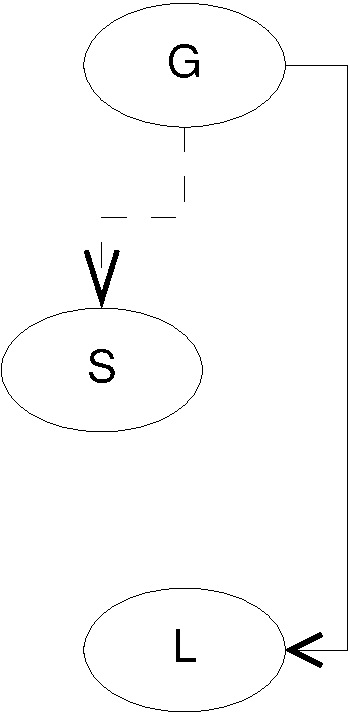
\includegraphics[width=1.5cm]{goto}
  \end{center}
&
\begin{itemize}
\item soit un programme P,
\item soit \n{g} un noeud du CFG de P correspondant à un  \verbtt{goto},
\item soit \n{l} le noeud correspondant au successeur de \n{g} (label du \verbtt{goto}),
\item soit P', le programme P dans lequel on remplace le \verbtt{goto}
par un ';' (NOP),
\item soit \n{g}' le noeud correspondant dans le CFG de P',
\item soit \n{s} le successeur lexical de \n{g}.
\end{itemize}
\bigskip
On veut qu'un noeud \n{a} ait une dépendance de contrôle sur \n{g}
\ssi \n{a} postdomine soit \n{g}, soit \n{s}, mais pas les deux.
\end{tabularx}
\end{monenv}
Examinons les différents cas~:
\begin{enumerate}
  \item si \n{s}=\n{l}, cela signifie que le \verbtt{goto} ne sert à rien,
    personne ne dépend donc de \n{g},
  \item si \n{l} postdomine \n{s}, \n{s} dépend de \n{g}, ainsi que tous les postdominateurs
    de \n{s} qui ne postdomine pas \n{l},
  \item si \n{l} ne postdomine pas \n{s},
  tous les \n{a} qui postdominent \n{s}, mais pas \n{l} ou l'inverse, dépendent de \n{g}.
\end{enumerate}

Donc, de manière générale, on peut calculer~:
$$
  \codpdc{g} = (\P{s} \cup \P{l}) - (\P{s} \cap \P{l})
$$
ce qui nous donne bien les noeuds atteints par l'une ou l'autre des branches,
mais pas par les deux.

On peut d'ailleurs montrer qu'on obtient la même chose que si on calcule \codpdc{g^*}
sur CFG$^*$ où CFG$^*$ est le CFG dans lequel le noeud \n{g} est remplacé par un
noeud \n{g^*} correspondant à une instruction
\verbtt{if (true) goto L;}\\



\section{Boucle infinie et exit}

Comme on l'a vu,
la plupart des définitions de dépendance de contrôle se basent
sur le CFG, la notion de postdominateurs, et utilisent l'hypothèse
que le CFG a un unique noeud de sortie \nE{} atteignable depuis tous les
autres points du graphe. Or, comme l'explique très bien \cite{ranganath04new},
cette hypothèse ne tient plus dans les programmes contenant
des boucles infinies ou des \verbtt{exit} (ou même des exceptions,
mais pour le langage C, nous n'avons pas le problème).
Cet article présente également avec beaucoup de détails
différents types de dépendances et des algorithmes pour les calculer,
mais il s'avère probablement trop complexe pour ce que l'on souhaite faire.\\

Le fait qu'une fonction n'atteigne pas forcement un point de sortie pose deux
problèmes différents~:
\begin{itemize}
  \item la préservation de la non-terminaison,
  \item le calcul des dépendances de contrôle pour les instructions
    n'ayant pas de chemin vers la sortie.
\end{itemize}

\subsection{Préservation de la non-terminaison}

La question qui se pose est de savoir s'il faut ajouter des dépendances de
contrôle sur les instructions qui, potentiellement, ne terminent pas.

\begin{exemple}
    \begin{tabular}{p{5.5cm}p{\dimexpr\linewidth-6.5cm}}
\begin{clisting}
while (f(x) > 0) x++;
L: y = 3;
\end{clisting}
&
Si l'on s'intéresse au calcul de {\tt y} en {\tt L}, on peut se demander si
cette instruction a une dépendance de contrôle sur la boucle,
car si dans certains cas, la boucle ne termine pas,
{\tt L} n'est pas atteint le même nombre de fois
dans le programme source P, et dans le programme P' dans lequel la boucle est
remplacée par un NOP.

\end{tabular}
\end{exemple}

Pour prendre en compte ce type de problème et permettre d'effectuer par la suite
des analyses sensibles à la non-terminaison ({\it non-terminaison sensitive}),
il faut ajouter des dépendances à toutes les instructions qui suivent
une construction qui peut ne pas terminer comme un appel de fonction,
ou une boucle dont on ne sait pas déterminer la terminaison.
Dans l'absolu, il faudrait aussi s'intéresser aux autres instructions qui ont
une terminaison anormale (\verbtt{Segmentation Fault} par exemple) mais il semble
raisonnable de considérer que ces instructions ne sont jamais présentes exprès,
et que leur absence doit être vérifiée par ailleurs.

\subsection{Postdominateurs généralisés}

\subsubsection{Définition}

En cas de boucle infinie, le CFG contient des noeuds pour lesquels
il n'existe pas de chemin vers la sortie.
Or, pour un tel noeud \n{a},
les postdominateurs tels que définis plus haut me peuvent pas être utilisé
pour déterminer les dépendances de contrôle.
En effet, on ne peut pas parler des instructions qui vont être
forcement exécutées entre \n{a} et \nE{} car il n'existe pas de telles traces.\\

La plupart des travaux existants travaillent dans ce cas sur un CFG augmenté
dans lequel le noeud \nE{} est ajouté, ainsi que des arrêtes pour le rendre
accessible. Outre le fait que certaines analyses n'aient pas besoin de cette
hypothèse, et qu'une telle modification vienne ``polluer'' le CFG,
il semble difficile (impossible ?) de ne pas ajouter
de dépendances parasites dans le cas des boucles infinies.\\

Pourtant, même si \n{a} est dans une boucle infinie,
on a intuitivement une notion de postdominateurs. On aimerait bien dire
qu'une instruction \n{b} postdomine une instruction \n{a} \ssi \n{b} appartient
à tous les chemins {\bf partant de \n{a}}, c'est-à-dire~:

\begin{definition}{postdominateurs généralisés}
$$ \n{b} \in \Pdi{a} \define \forall t \in \allmch{a, -}, \n{b} \in t $$
\end{definition}


On ne considère donc plus uniquement les chemins qui atteignent la sortie,
mais toutes les traces d'exécution possible.


\subsubsection{Méthode de calcul}


Intuitivement, si on souhaite connaître tous les noeuds qui ont b comme
postdominateurs en considérant tous les chemins,
on peut calculer les ensembles suivants~:
$$
E_b (a) = \left\{
\begin{array}{ll}
  {b} & \text{si } b = a\\
  \bigcap_{s \in \succ{a}} E_b(s) & \text{sinon.}
\end{array}\right.
$$
en partant d'ensembles initialement vides.
Ce calcul termine car il est croissant.

A la fin du calcul, on a :
$$
  \forall b, E_a (b) = \{ a \} \vee E_a (b) = \bot
$$
et $E_a (b) = \{ a \}$ veut bien dire que $a$ est dans tous les chemins entre
$b$ et $a$.\\

On peut faire ce calcul pour tous les points du CFG, et faire l'union de tous
les résultats obtenus~:
$$
\Pdi(a) = \bigcup_{b \in CFG} E_b(a)
$$
Bien sûr, ce n'est pas la manière la plus efficace de faire le calcul,
mais on voit trivialement que c'est le résultat que l'on souhaite obtenir.\\

Il suffit maintenant de trouver un calcul équivalent,
moins coûteux, mais qui termine néanmoins...

En fait, il suffit de faire directement
l'union des résultats au fur et à mesure du calcul,
mais comment prouver la terminaison~?

\subsubsection{Discussion}

On remarque que cette définition ne donne pas
les mêmes postdominateurs que précédemment
dès qu'il y a une boucle dans le CFG, même qui la sortie \nE{} est accessible
depuis tous les noeuds,
car il existe alors un chemin possible qui consiste à boucler indéfiniment.
Par conséquent, les instructions situées après la boucle ne postdomine pas les
instructions de la boucle puisqu'il existe un chemin pour lequel on y passe pas.
Cela traduit le fait que l'exécution de ces instructions dépend du fait que la
boucle termine...

Si on utilise cette définition des postdominateurs pour calculer des dépendances
de contrôle, on va donc ajouter des liens entre la boucle et tout ce qui suit.
Ces nouvelles dépendances traduisent la possible non-terminaison de la boucle,
et peuvent donc servir dans le cadre d'une analyse préservant la non-terminaison
comme on l'a vu précédemment.
Mais on ne souhaite pas nécessairement ajouter toutes ces dépendances,
car en pratique, on peut montrer par ailleurs que la plupart des boucles
d'un programme terminent.

\subsection{Postdominateurs augmentés}\label{sec-pda}

On peut essayer de faire un mélange des postdominateurs classiques et des
postdominateurs généralisés en supposant que toutes les boucles ayant une
sortie se terminent (attention : on considère pour l'instant qu'il y a un chemin
possible entre cette sortie et \nE), mais en considérant néanmoins
les traces infinies dans les cas où une boucle n'a pas de sortie.

\begin{definition}{postdominateurs augmentés}
$$
\Pda{a} = \left\{
\begin{array}{ll}
\{ b | \forall t \in \allmch{a, -}, b \in t \}
  & \text{si } \allch{a, \nE} = \{\}\\
\{ b | \forall t \in \allmch{a, \nE}, b \in t \}
  & \text{sinon.}
\end{array}\right.
$$
\end{definition}


\subsubsection{Méthode de calcul}

\newcommand{\ToRet}[1]{\ensuremath{\mathit{ToRet}(\n{#1})}}

Pour faire ce calcul, il faut être capable de distinguer les chemins qui mènent
à \nE{} des autres.
On note \ToRet{a} la propriété qui dit que \n{a} a un chemin vers \nE.

Après un calcul classique des postdominateurs (en partant de \nE),
les postdominateurs des noeuds tels que  \ToRet{a} sont établis.
Reste à calculer l'information pour les autres noeuds, c'est-à-dire ceux qui
ont les postdominateurs à $\top$.

Pour ceux-là, on fait un calcul similaire~:
$$
\Pda{x} = \{\n{x}\} \bigcup \bigcap^a_{s \in \succ{x}} \Pda{s}
$$
en redéfinissant simplement l'intersection utilisée de la façon suivante~:
$$
\Pda{a} \cap^a \Pda{b} =  \left\{
\begin{array}{ll}
  \Pda{a} \cap \Pda{b} & \text{si } \ToRet{a} = \ToRet{b}\\
  \Pda{a}              & \text{si } \ToRet{a} \et \neg\ToRet{b}\\
  \Pda{b}              & \text{si } \neg\ToRet{a} \et \ToRet{b}\\
\end{array}\right.
$$


\subsubsection{Discussion}

On remarque qu'avec cette définition, il existe des noeuds \n{a} tels que~:
$$
\succ{a} = \{\n{s1}, \n{s2}\} \et \Pda{a} \neq \Pda{s1} \cap \Pda{s2}
$$
dans le cas où on atteint la sortie à partir de l'un des successeurs, mais pas
de l'autre.

Par exemple, si on considère un noeud \n{c} correspondant à un {\sc IF}
dont l'une des branche est une boucle infinie et que l'autre permet d'atteindre
la sortie, la boucle infinie dépendra de \n{c}, alors que l'accès à la sortie
n'en dépendra pas.


\section{En résumé}

Pour calculer les dépendances de contrôle, on commence donc par calculer les
postdominateurs augmentés définis en \S\ref{sec-pda}.
Puis, pour chaque saut, on calcule ses co-dépendances de contrôle de la façon
suivante~:

\begin{itemize}
  \item pour un {\sc IF},
    on applique la définition donné en \S\ref{sec-dpdc-if},
    c'est-à-dire~:
$$
\codpdc{c} = \bigcup_{ \n{s} \in \succ{c}} \Pda{s} - \Pda{c}
$$

  \item pour un saut inconditionnel (\verbtt{goto}, \verbtt{break}, etc),
    comme mentionné en \S\ref{sec-dpdc-goto}, on calcule~:
$$
\codpdc{g} = (\Pda{s} \cup \Pda{l}) - (\Pda{s} \cap \Pda{l})
\text{  où } \left\{\begin{array}{l}
\n{s} = \succl{g} \\
\n{l} = \succ{g}
\end{array}\right.
$$
Si on considère \n{s} et \n{l} comme deux pseudo-successeurs de \n{g},
les pseudo-postdominateurs de \n{g} sont donnés par
$(\Pda{s} \cap \Pda{l})$, et on retrouve bien la formule précédente.

  \item pour les boucles, comme dans CIL, elles sont toutes infinies,
on traite la séquence \verbtt{while(1) S;}
comme si on avait \verbtt{L : S; goto L;}

\end{itemize}
